In this section, we empirically evaluate STOIC's performance when executing machine learning applications. We compare its use of multiple runtimes
versus solely using a single runtime for all batches.  In the sections
that follow, we first describe 
the machine learning application that we consider. We then
present our experimental setup and results. 

\subsection{Benchmark Application and Dataset}

We evaluate STOIC using an image processing application that classifies animal images from a wildlife monitoring system called ``Where's The Bear" (WTB)~\cite{ref:wtb}. ``Where's The Bear" is an end-to-end distributed data acquisition and analytics system that implements an IoT architecture and edge cloud. Our application makes inferences for each photo taken by deployed camera traps in Sedgwick Natural Reserve using a convolutional neural network (CNN)~\cite{ref:cnn}.  We train the model using labeled images from the WTB dataset. Technically, the application employs Tensorflow and Scikit-learn~\cite{ref:scikit} to implement 
image classification.  

In total, there are five classes that we consider in the CNN model training: Bird, Fox, Rodent, Human and Empty. Since class size is unbalanced due to frequencies of animal occurrances, we up-sample minority classes (e.g. fox) using 
the Keras ImageDataGenerator~\cite{ref:keras}.  Doing so ensures that the classification model is not biased. We resize every image in the WTB dataset to $1920 \times 1080$, and for each class, the dataset contains 251 images used to train the CNN model. Once model training is complete, the application stores this model in hdf5 format in cloud storage at both edge cloud (disk storage) and Nautilus (a shared volume in a Ceph file system).

\subsection{Performance Evaluation}

\begin{table}[t] \centering 
\scriptsize
\resizebox{\columnwidth}{!}{
\begin{tabular}{|c|c|c|c|c|} 
\hline
& \textbf{Mean $T_r$ (sec)} & \textbf{Stdev. $T_r$ (sec)} & \textbf{Mean $T_p$ (sec)} & \textbf{Stdev. $T_p$ (sec)}\\
\hline
edge & 108.88 & 1.65 & 108.88 & 1.65 \\
\hline
cpu & 100.0 & 4.93 & 86.99 & 4.92 \\
\hline
gpu1 & 98.90 & 4.03 & 50.65 & 4.05 \\
\hline
gpu2 & 106.29 & 5.53 & 39.21 & 5.55\\
\hline
\textbf{STOIC} & \textbf{97.73} & \textbf{3.13} & \textbf{50.49} & \textbf{3.11} \\
\hline
\end{tabular}
}
\caption{Mean and stdev of total response time~($T_r$) and processing time~($T_p$) of 40-image batch: STOIC schedules tasks onto the runtime (\textit{gpu1}) that has the least total response time~($T_r$).
\label{tab:validation}}
\end{table}

We first test the efficacy of STOIC by processing an image batch of fixed size at four runtimes individually and then compare them with STOIC. To make the result reliable, we again conduct the experiment 10 times and list the mean and standard deviation of total response time~($T_r$) and processing time~($T_p$) in Table~\ref{tab:validation}. We can observe from Table~\ref{tab:validation} that STOIC schedules 40-image batch to \textit{gpu1} runtime, based on its prediction that  \textit{gpu1} would have the least total response time~($T_r$). One important observation is that \textit{gpu2} runtime has even lower processing time~($T_p$) than \textit{gpu1}, but STOIC disregard \textit{gpu2} in this scenario, because its gain in processing time~($T_p$) does not compensate for its lengthy deployment time~($T_d$) on Nautilus cloud.

\begin{figure}[t] \centering 
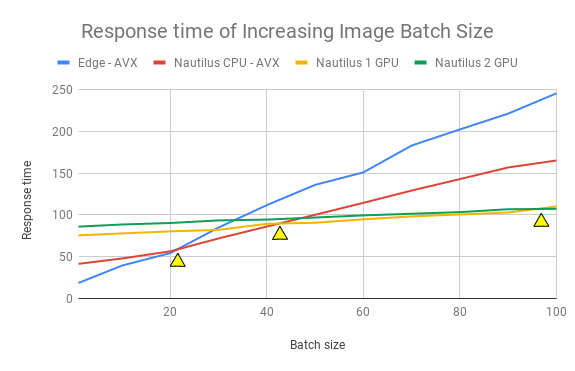
\includegraphics[scale=0.32]{response-time}
\caption{Total Response Time~($T_r$) of image batches of growing sizes: The x-axis represents the batch size, while the y-axis is the total response time~($T_r$). STOIC, which is depicted in the blue dashed line, schedules the task on the runtime with the least total response time.  
\label{fig:response-time}}
\end{figure}

We next test STOIC by processing a series of image batches of growing sizes on the four runtimes and STOIC. Figure~\ref{fig:response-time} shows their total response times. The x-axis is the size of the image batch and the y-axis is the total response time~($T_r$) in seconds. The red curve show that latency
increases linearly over the \textit{edge} runtime.  The yellow curve 
shows the performance of the \textit{cpu} runtime in the Nautilus cloud. 
We observe that its slope is more moderate than \textit{edge} runtime since CPUs in nodes of Nautilus cloud are usually more powerful than those in the edge cloud. The pink and green curve represent the \textit{gpu1} and \textit{gpu2} runtimes, respectively, and they intersect at a batch size of 95, at which STOIC would switch the deployment of task from \textit{gpu1} to \textit{gpu2}. The blue dashed line depicts the total response time~($T_r$) of STOIC, which is able to schedule a series of tasks to the runtime with the least latency. According to such result, STOIC improves system performance by determining the best runtime
for the given task dynamically.


%\subsection{Empirical Experiment}


% \begin{table}[t]
%     \centering
%     \scriptsize

\begin{tabular}{|c|c|c|c|c|c|} 
\hline
\textbf{Runtimes}& \textbf{edge} & \textbf{cpu} & \textbf{gpu1} & \textbf{gpu2} & \textbf{STOIC} \\
\hline
Avg. $T_r$ (sec) & 2842.58 & 2065.59 & 2173.98 & 2201.02 & 1931.64 \\
\hline
Speed-up (\%) & 32.05 & 6.48 & 11.15 & 12.24 & N/A \\
\hline
\end{tabular}

%     \caption{\textbf{Average total response time~($T_r$) and speed-up on 24-hour dataset}: Comparing with four single runtimes, STOIC achieves lowest average latency and speed-up ranging from 6.48\% to 32.05\%. }
%     \label{tab:24-batches}
% \end{table}


We next perform an empirical evaluation of STOIC by comparing the 
total response time~($T_r$) of multiple image batches of different
sizes across the four single runtimes and STOIC.  To accelerate the 
repetitive experiment, we developed a simulator to generate image batches based on the frequency distribution of the WTB dataset. 

According to 2016 WTB dataset, the size of image batch fits to normal distribution $\mathbf{N}(\mu = 42.75, \sigma^2 = 39.5)$. Thus, the simulator generates 24 image batches in the edge controller to emulate streaming data in one day from open field camera traps. To conduct an unbiased evaluation, we seed the simulator to make these 24 image batches consistent across all runtimes and STOIC. 

\begin{figure}[t] \centering 
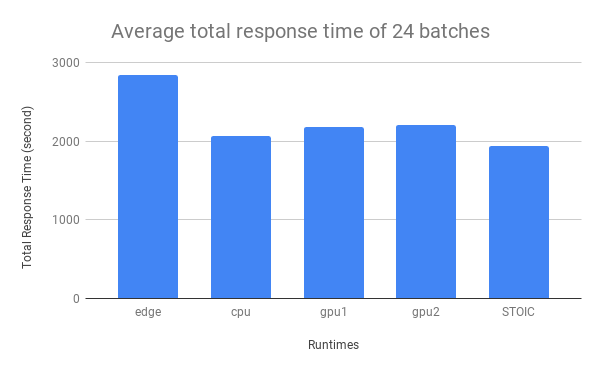
\includegraphics[scale=0.42]{figures/24-batches}
\caption{Average total response time~($T_r$) on the 24-hour dataset: The x-axis represents runtimes, while the y-axis represents the average total response time~($T_r$) by STOIC and four other runtimes on the 24-hour dataset. The data labels on columns are specific numbers of $T_r$. The seeded simulator generates the 24-hour batch sizes from the distribution of historical data. 
\label{fig:24-batch}}
\end{figure}

To ensure the validity of the outcome, we run each experiment 10 times for each runtime scenario and report the average value. Figure~\ref{fig:24-batch} shows the average total response time~($T_r$) for STOIC and the four individual runtimes. STOIC achieves the lowest average latency versus the four other single runtimes.  STOIC reduces total response time~($T_r$) by 32.05\% (versus \textit{edge}), 6.48\% (versus \textit{cpu}), 11.15\% (versus \textit{gpu1}) and 12.24\% (versus \textit{gpu2}) respectively. According to such a result, we conclude that STOIC outperforms single-runtime scheduling mechanism on the empirical datasets and real-world machine learning applications.
